\documentclass[11pt]{article}
\usepackage[a4paper,margin=2.6cm]{geometry}
\usepackage[T1]{fontenc}
\usepackage[utf8]{inputenc}
\usepackage{lmodern}
\usepackage{booktabs}
\usepackage{graphicx}
\usepackage{amsmath}
\usepackage{multirow}
\usepackage{caption}
\usepackage[round]{natbib}
\usepackage[hidelinks]{hyperref}
\usepackage{xcolor}
\captionsetup{font=small,labelfont=bf}
\graphicspath{{figures/}{../results/}}

\newcommand{\todoresult}[1]{\textcolor{red!70!black}{[#1]}}
\newcommand{\cometda}{\textsc{wmt22-comet-da}}
\newcommand{\kiwi}{\textsc{wmt22-cometkiwi-da}}

\title{Length Sensitivity of Learned MT Metrics:\\
Encoder Alignment, Domain Adaptation, and Training-Mix Composition}
\author{Adle Ben Salem\\ \small Inria Paris}
\date{August 2026 --- working report}

\begin{document}
\maketitle

\begin{abstract}
Learned MT metrics such as COMET are trained on single sentences.
In practice they are applied to paragraphs and documents.
We study what this mismatch costs, in three steps.
First, we isolate length itself.
We build blocks of $k$ consecutive FLORES+ sentences and ask whether encoders still separate a translation from a copy with a single injected error.
COMET's encoder drops below chance already at $k{=}3$; sentence aligners (LaBSE, E5) degrade far more slowly.
A matched-core design shows the drop persists with meaning-free filler, so it is a property of the representation, not of content.
Second, we revisit domain adaptation on Bio-MQM.
Fine-tuning \cometda{} in domain moves Pearson slightly ($+0.018$) and rank correlation not at all, and leaves encoder representations essentially unchanged.
Third, we continue \cometda{} and \kiwi{} on WMT training mixes that vary only the fraction of single-sentence data, at constant total size.
We document a subtle training-pipeline failure that invalidated a first 36-arm sweep, and a corrected protocol with an identical budget in every arm.
We evaluate the retrained metrics on sentence-level, aggregated, and natively long test sets, on MetaDocEval discourse perturbations, and on the block-alignment task.
The corrected sweep is running; this report will be updated with its results.
\end{abstract}

\section{Introduction}

COMET-style metrics dominate MT evaluation.
They are regressors on top of a multilingual encoder, trained on human judgments of single sentences.
Yet users score paragraphs and documents with them.
Three questions follow.

\textbf{Q1.} Does input length \emph{by itself} degrade the encoder signal that the metric relies on?
We answer this with controlled alignment tasks on FLORES+ (Section~\ref{sec:isolation}).

\textbf{Q2.} What does fine-tuning on a new domain actually change?
We reproduce the Bio-MQM setting of \citet{zouhar2024biomqm} (Section~\ref{sec:bio}).

\textbf{Q3.} If we continue training the metric on longer inputs, what does that buy, and what does it cost at the sentence level?
We run a controlled sweep over the sentence fraction of the training mix (Section~\ref{sec:mix}).

Throughout, ``COMET'' means \cometda{} \citep{rei2022comet} and ``CometKiwi'' means the reference-free \kiwi{} \citep{rei2022cometkiwi}.
Both use an XLM-R large encoder \citep{conneau2020xlmr}.

\section{Q1: length in isolation --- block alignment on FLORES+}
\label{sec:isolation}

\subsection{Setup}

FLORES+ \citep{nllb2022,oldi2024flores} provides sentence-aligned articles in many languages.
A \emph{block} is $k$ consecutive sentences of one article, concatenated; blocks do not overlap.
We use $k \in \{2,3,4,5\}$, languages de/es/fr/ru with English pivot, direction en$\to$xx.
Per language there are 846 blocks at $k{=}2$ and 141 at $k{=}5$.

We inject exactly one error into one sentence of a block, following the xSIM++ taxonomy \citep{chen2023xsimpp}: causality (negation, antonym, modality), entity replacement, and number changes.
Each perturbed block differs from its source block by a single edit.

We compare five frozen encoders by cosine similarity: COMET's encoder, the same encoder after Bio-MQM fine-tuning (Section~\ref{sec:bio}), mean-pooled XLM-R large, LaBSE \citep{feng2022labse}, and multilingual E5 \citep{wang2022e5}.
Three probes separate the failure modes:

\begin{itemize}
\item \textbf{block-xSIM++}: retrieval over the full pool of true and perturbed blocks. \emph{xsim} error uses true blocks only (pure alignment); \emph{xsim++} error adds the perturbed copies; the \emph{detection rate} is $P[\cos(q,\text{gold}) > \cos(q,\text{perturbed})]$, chance $0.5$.
\item \textbf{fixed-pool duel}: every retrieval is one gold block against exactly $D$ single-error negatives, averaged over all subsets in closed form. Task difficulty is identical at every $k$; only length varies. Chance error is $D/(D{+}1)$.
\item \textbf{matched core}: the \emph{same} core sentence (with its perturbed variants) is embedded in filler of total length $L \in \{60,120,240,480\}$ XLM-R tokens. Filler types: \emph{inert} (a repeated neutral phrase), \emph{neutral} (unrelated FLORES sentences), \emph{distractor} (same-article sentences), \emph{natural} (contiguous corpus text). Any change across $L$ is attributable to length, never to content. All inputs stay under the 512-token limit, so truncation plays no role.
\end{itemize}

\subsection{Results}

\paragraph{Alignment is easy; error detection is not.}
Classic xsim error is near zero for COMET, LaBSE and E5 at every $k$.
The metrics-relevant signal is elsewhere: with perturbed copies in the pool, COMET's retrieval collapses (Table~\ref{tab:blockxsim}).
Its detection rate falls below chance at $k{=}3$.
The dedicated aligners degrade too, but stay far above chance.
Bio-MQM fine-tuning changes nothing.

\begin{table}[t]
\centering\small
\begin{tabular}{l cccc cccc}
\toprule
& \multicolumn{4}{c}{xsim++ error $\downarrow$} & \multicolumn{4}{c}{detection rate $\uparrow$ (chance .50)}\\
\cmidrule(lr){2-5}\cmidrule(lr){6-9}
encoder & $k{=}2$ & $k{=}3$ & $k{=}4$ & $k{=}5$ & $k{=}2$ & $k{=}3$ & $k{=}4$ & $k{=}5$\\
\midrule
COMET encoder        & .72 & .87 & .94 & .98 & .59 & .47 & .40 & .34\\
\;+ Bio-MQM ft.      & .72 & .87 & .94 & .98 & .58 & .46 & .39 & .34\\
XLM-R mean           & .87 & .93 & .97 & .98 & .51 & .48 & .46 & .44\\
LaBSE                & .27 & .48 & .63 & .76 & .93 & .89 & .87 & .83\\
E5                   & .24 & .44 & .60 & .73 & .94 & .91 & .89 & .85\\
\bottomrule
\end{tabular}
\caption{Block-xSIM++ on FLORES+, mean over de/es/fr/ru. One injected error per block. COMET's encoder loses the error as $k$ grows; aligners keep it.}
\label{tab:blockxsim}
\end{table}

\paragraph{The pool is not the cause.}
In block-xSIM++ the candidate pool grows with $k$.
The duel removes this confound: with a fixed number of negatives per decision, COMET is at or below chance at every $k$ and still degrades monotonically (duel error at $D{=}4$: $.79 \to .95$ from $k{=}2$ to $k{=}5$; chance $.80$).
LaBSE and E5 sit far above chance at all $k$ ($.27 \to .53$ and $.22 \to .48$).

\paragraph{Length alone is sufficient.}
The matched-core results (Figure~\ref{fig:matchedcore}) make the strongest point.
With \emph{inert} filler --- a repeated, meaning-free phrase --- COMET's detection falls from $.73$ at $L{=}60$ to $.47$ at $L{=}120$, below chance.
No semantics is added; only length.
With natural filler the picture is the same ($.78 \to .40$).
LaBSE never falls below $.88$ and E5 never below $.82$, at any $L$ and filler type.
As a scalar summary, COMET loses $0.11$ detection per doubling of $L$ with inert filler ($\mathrm{LSI} = -.105$, 95\% CI $[-.115, -.095]$) and $0.12$ with natural filler; LaBSE and E5 lose at most $0.02$--$0.04$ and never cross the $.75$ mark that defines $L_{50}$.
A layer-wise probe of XLM-R shows the error signal is progressively lost toward the top layers and pooling; with natural filler it is still present in the early and middle layers, while with inert filler it fades earlier.
The top-layer embedding of the whole input barely moves when the core is perturbed (cosine $\ge .97$ to the clean version): the negatives are geometrically almost indistinguishable.

\begin{figure}[t]
\centering
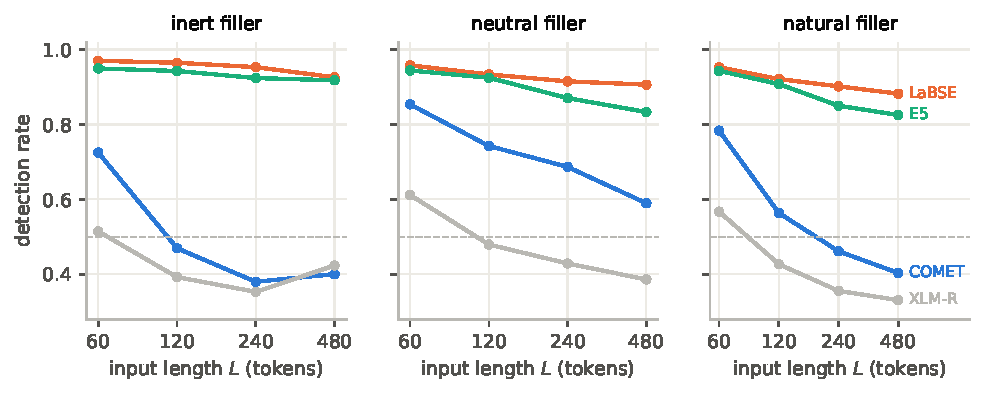
\includegraphics[width=.95\linewidth]{matched_core_report.pdf}
\caption{Matched-core detection vs.\ total input length $L$ (XLM-R tokens), per filler type, mean over de/es/fr/ru. The same core sentence and the same single error at every $L$; only filler length varies. Dashed line: chance.}
\label{fig:matchedcore}
\end{figure}

\paragraph{Reading.}
Sentence-level error sensitivity of COMET's encoder does not survive concatenation.
The failure is representational and driven by length itself.
This motivates Q3: can training on longer inputs restore the signal?

\section{Q2: domain adaptation on Bio-MQM}
\label{sec:bio}

This part is secondary; it reproduces the setting of \citet{zouhar2024biomqm} and provides the fine-tuned checkpoint used above.

\subsection{Setup}

Bio-MQM provides sentence-level MQM annotations in the biomedical domain, 10 language pairs.
We map error severities to penalties (minor $-1$, major $-5$, critical $-25$), average over annotators, z-normalise per language pair and squash by a sigmoid.
The paper's dev documents form our training set, its test documents our validation set.
We continue \cometda{} with a conservative schedule (encoder LR $5\times10^{-7}$, head LR $10^{-5}$, effective batch 64).

\subsection{Results}

\begin{table}[t]
\centering\small
\begin{tabular}{l cc cc}
\toprule
& \multicolumn{2}{c}{Pearson} & \multicolumn{2}{c}{Kendall $\tau$}\\
\cmidrule(lr){2-3}\cmidrule(lr){4-5}
LP & base & fine-tuned & base & fine-tuned\\
\midrule
de-en & .279 & .339 & .354 & .352\\
en-de & .485 & .560 & .450 & .454\\
en-es & .293 & .330 & .329 & .326\\
en-fr & .433 & .494 & .386 & .382\\
en-ru & .571 & .525 & .351 & .352\\
es-en & .451 & .444 & .343 & .340\\
fr-en & .465 & .459 & .347 & .346\\
ru-en & .470 & .437 & .288 & .279\\
\midrule
mean  & .431 & .448 & .356 & .354\\
\bottomrule
\end{tabular}
\caption{Sentence-level correlation with human MQM on Bio-MQM test documents: \cometda{} before and after in-domain fine-tuning.}
\label{tab:bio}
\end{table}

Fine-tuning helps calibration a little and ranking not at all (Table~\ref{tab:bio}): mean Pearson $+0.018$, mean Kendall $-0.002$.
Representation probes tell the same story.
Frozen-probe accuracies on XNLI, PAWS-X and news classification, and full fine-tune accuracies on XNLI and PAWS-X, match the base COMET encoder within $\pm 0.01$.
What moves representations is COMET training itself, not the domain adaptation on top (frozen-probe XNLI: XLM-R $.393$, COMET $.445$).
This is consistent with the paper's core finding that fine-tuned metrics gain little robustness from such adaptation.

\paragraph{Open items.}
zh pairs are not yet in our correlation runs.
A side-by-side table against the published per-LP numbers, under the paper's exact score aggregation, remains to be built.
WMT25 provides additional biomedical-adjacent data that could extend this comparison.

\section{Q3: training-mix composition at constant budget}
\label{sec:mix}

\subsection{Data: three pools, one schema}

We build three training pools with a common COMET schema (src, mt, ref, score):

\begin{itemize}
\item \textbf{sent}: WMT22 MQM single segments (en-de, en-ru, zh-en) \citep{freitag2022wmt22}; 59{,}144 rows.
\item \textbf{agg}: the same segments, concatenated in windows of $k \in \{2,3,4,6\}$ consecutive same-document segments; the window score is the mean segment score; 160{,}377 rows.
\item \textbf{native}: WMT25 general-MT human evaluation \citep{kocmi2025wmt25}; the scored unit is a whole document ($k{=}0$); only documents with a reference are kept, so the reference-based and reference-free arms train on identical rows; 42{,}558 rows.
\end{itemize}

Scores are z-normalised per (source, LP) and sigmoid-squashed; this is monotone, so rank correlations are unaffected.
Splits are document-disjoint.

\subsection{Mixes and arms}

Each mix holds exactly 24{,}000 rows.
The sentence fraction $f \in \{0, 10, 20, 40, 60, 80, 100\}\%$ sets the share of single sentences; the remaining mass is split 50/50 between aggregated windows and native documents.
Two ablations pin the origin of the long mass at $f{=}0$: \emph{frac000nat} (all native) and \emph{frac000agg} (all aggregated).
Pools are shuffled once (seed 42) and mixes take prefixes, so mixes differ only by prefix length.
Crossed with two base metrics (\cometda{}, \kiwi{}) and two encoder regimes (unfrozen vs.\ frozen encoder), this gives $2 \times 9 \times 2 = 36$ arms.

\paragraph{A known confound.}
The sent/agg pools cover 3 language pairs, the native pool 13, with almost no overlap.
Moving $f$ therefore also moves the language distribution.
We keep this explicit and analyse per language pair where it matters.

\subsection{The first sweep did not measure composition}
\label{sec:bug}

A first 36-arm sweep (2026-08-17) produced validation curves that rise and then fall (Figure~\ref{fig:bell}), and an arm ranking that turned out to be an artefact.
The cause was in file handling, not in the mixes.
COMET selects one training file per epoch (\texttt{train\_data[epoch \% len]}), and the trainer never rebuilt the dataloader.
Passing one CSV per language pair therefore trained every arm on \emph{its first file only}: between 205 and 6{,}940 rows instead of 24{,}000.
Two fatal confounds followed.
Training budgets differed by a factor of ${\sim}34$ across arms.
And the arms trained on different language pairs.
An earlier Bio-MQM version of the sweep (2026-08-14) had the same defect, hidden there by a constant file count per arm.

The bell shape itself has a second, independent cause: early stopping monitored validation Kendall with patience 20 on tiny epochs, so \emph{every} run ended exactly 20 evaluations past its peak, deep into overfitting.
The Bio-MQM runs lose up to $0.076$ Kendall from peak to final checkpoint.

\begin{figure}[t]
\centering
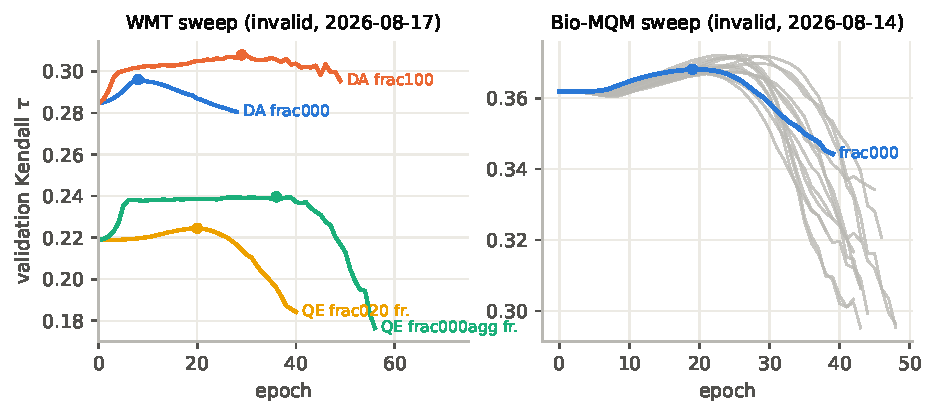
\includegraphics[width=.95\linewidth]{wandb_bell.pdf}
\caption{Validation Kendall $\tau$ during the two invalid sweeps. Dots mark peaks; every run ends exactly 20 evaluations later (early-stopping patience). Left: representative WMT arms. Right: all Bio-MQM arms (grey), one highlighted.}
\label{fig:bell}
\end{figure}

\paragraph{Corrected protocol.}
Every arm now trains on its mix's single concatenated CSV: one epoch is the whole 24{,}000-row mix in every arm.
The budget is fixed grid-wide: max 6 epochs ($\le 4{,}500$ optimizer steps at effective batch 32), validation once per epoch, patience 3, and model selection by best validation Kendall, never by the last checkpoint.
Three guards prevent regressions: the config generator refuses multi-file training data; the training library warns when files would be ignored; evaluation caches are invalidated by checkpoint fingerprint.
Checkpoints from before the correction are quarantined and excluded.

\subsection{Evaluation lenses}

\begin{itemize}
\item \textbf{Per-$k$ correlation.} Kendall $\tau$ against human scores on: WMT22 sentence and aggregated-window sets ($k \in \{1,2,3,4,6\}$); natively long WMT25 document sets; and held-out WMT23/24 paragraph sets never seen in training.
\item \textbf{MetaDocEval} \citep{dahan2026metadoceval}. Contrastive accuracy $P[\text{score(orig)} > \text{score(perturbed)}]$ over nine document-level perturbations, scored with SLIDE-style windows \citep{raunak2024slide} of $w \in \{1,3,6,9\}$ segments. \texttt{sentence\_splitting} is quality-preserving by design; its ``accuracy'' is a false-positive rate. Two categories are smaller than the upstream README advertises (verified against the data); all results use measured counts.
\item \textbf{Block alignment} (Section~\ref{sec:isolation}) with the retrained encoders: does mix training restore single-error detection in long blocks?
\end{itemize}

\subsection{Baselines}

Figure~\ref{fig:baselinetau} shows the released metrics under the per-$k$ lens.
Both track human judgment best on single sentences ($\tau = .397$ for COMET-DA, $.331$ for CometKiwi, mean over WMT22 pairs).
On natively long documents both drop sharply ($.272$ and $.239$).
Aggregated windows sit in between and recover with $k$; this is expected, since averaging segment scores denoises the target.

\begin{figure}[t]
\centering
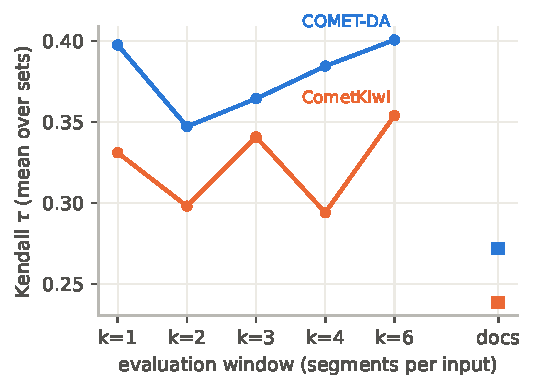
\includegraphics[width=.5\linewidth]{baseline_tau_vs_k.pdf}
\caption{Baseline Kendall $\tau$ by evaluation window. Lines: WMT22 aggregated windows. Squares: natively long documents (WMT23--25), the hard case.}
\label{fig:baselinetau}
\end{figure}

On MetaDocEval (Figure~\ref{fig:mdebase}), both baselines detect structural perturbations near ceiling at $w{=}1$ and dilute as context grows.
For the lexical categories (tense, lexical consistency, conjunction), COMET-DA starts higher and \emph{decays} with $w$; no baseline genuinely improves with context.
This is the paper's central negative result, and the question for the sweep is whether any retrained arm climbs instead of decaying.

\begin{figure}[t]
\centering
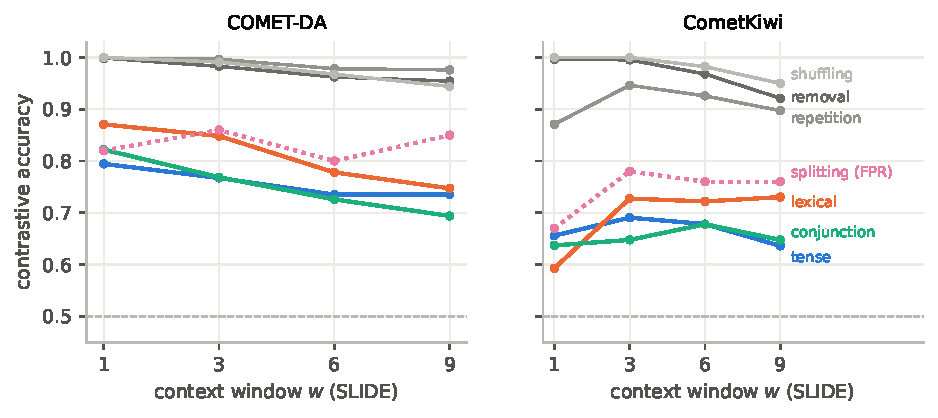
\includegraphics[width=.95\linewidth]{metadoceval_base.pdf}
\caption{MetaDocEval baselines: contrastive accuracy vs.\ context window $w$, micro-averaged per category. Grey: structural perturbations. Dotted: splitting, a false-positive rate. Dashed line: chance.}
\label{fig:mdebase}
\end{figure}

\subsection{Corrected sweep: first wave}
\label{sec:wave1}

Following the correction, we first train the eight arms that answer the headline question: $f \in \{0, 100\}\% \times$ \{DA, QE\} $\times$ \{frozen, unfrozen\}.
Startup checks confirm each arm loads exactly one 24{,}000-row file and the shared budget.
%% RESULTS-WAVE1-PLACEHOLDER: per-k table, MetaDocEval table, block-xSIM for wave-1 arms.
\todoresult{Training is running at the time of writing (jobs 5220084--5220091). Results will be inserted here.}

\subsection{Analysis plan}

Pre-specified, per arm and lens:
$\Delta\tau$ at $k{=}1$ vs.\ the arm's own base metric (forgetting);
the smallest $f$ that recovers baseline sentence-level $\tau$ (restoration point);
the slope of $\tau$ vs.\ $\log_2 k$ (length profile);
frozen-vs-unfrozen contrast (does the effect live in the encoder?);
DA-vs-QE contrast (does reference anchoring matter?);
MetaDocEval accuracy vs.\ $w$ (real discourse competence vs.\ rescaling).
Uncertainty: bootstrap over documents, never over windows, 1{,}000 resamples.

\section{Discussion}

Three results are already stable.
First, COMET's length problem is not (only) a data problem: the encoder itself stops separating a single error once the input grows, even with meaning-free filler.
Second, cheap fixes at the fine-tuning level are weak: in-domain adaptation barely moves representations, and its correlation gains are calibration, not ranking.
Third, measuring the effect of training composition is easy to get wrong: our first sweep silently trained every arm on a fraction of its data, and its ``findings'' reproduced the budget ranking.
Constant-budget design, single-file epochs and best-checkpoint selection are prerequisites, not details.

What the corrected sweep can decide: whether long-text training buys genuine document-level competence (MetaDocEval accuracy that rises with $w$; block detection that survives $k$) or only a rescaled score, and how much sentence data must stay in the mix.

\section{Conclusion}

We isolated length as a failure driver of COMET's encoder, quantified the limits of domain fine-tuning, and set up a corrected, constant-budget sweep over training-mix composition.
The first corrected wave is training.
The report will be updated with its per-$k$, MetaDocEval and block-alignment results.

\paragraph{Limitations.}
One seed per arm; bootstrap CIs quantify sampling noise, not seed noise.
The sent/agg vs.\ native pools differ in language coverage; $f$ moves both composition and language distribution.
Aggregated windows use mean segment scores as targets; the mean is itself a modelling choice, which MetaDocEval's contrastive design does not depend on.
Matched-core numbers use four languages and 120 cores per language; the layer probe is a reduced grid (de/fr, two filler types).

\begin{thebibliography}{20}\small

\bibitem[Burchell et al.(2024)]{oldi2024flores}
L.~Burchell, J.~Maillard, A.~Anastasopoulos, C.~Federmann, P.~Koehn, S.~Wang.
\newblock Findings of the WMT 2024 Shared Task of the Open Language Data Initiative.
\newblock WMT 2024.

\bibitem[Chen et al.(2023)]{chen2023xsimpp}
M.~Chen, K.~Heffernan, O.~\c{c}elebi, A.~Mourachko, H.~Schwenk.
\newblock xSIM++: An Improved Proxy to Bitext Mining Performance for Low-Resource Languages.
\newblock ACL 2023.

\bibitem[Conneau et al.(2020)]{conneau2020xlmr}
A.~Conneau et al.
\newblock Unsupervised Cross-lingual Representation Learning at Scale.
\newblock ACL 2020.

\bibitem[Dahan et al.(2026)]{dahan2026metadoceval}
N.~Dahan, R.~Bawden, F.~Yvon.
\newblock MetaDocEval: A Contrastive Framework for Evaluating Machine Translation Metrics at the Document-Level.
\newblock EAMT 2026. HAL: hal-05663019.

\bibitem[Feng et al.(2022)]{feng2022labse}
F.~Feng, Y.~Yang, D.~Cer, N.~Arivazhagan, W.~Wang.
\newblock Language-agnostic BERT Sentence Embedding.
\newblock ACL 2022.

\bibitem[Freitag et al.(2022)]{freitag2022wmt22}
M.~Freitag et al.
\newblock Results of WMT22 Metrics Shared Task: Stop Using BLEU -- Neural Metrics Are Better and More Robust.
\newblock WMT 2022.

\bibitem[Kocmi et al.(2025)]{kocmi2025wmt25}
T.~Kocmi et al.
\newblock Findings of the WMT25 General Machine Translation Shared Task: Time to Stop Evaluating on Easy Test Sets.
\newblock WMT 2025.

\bibitem[NLLB Team(2022)]{nllb2022}
NLLB Team, M.~R.~Costa-juss\`a, et al.
\newblock No Language Left Behind: Scaling Human-Centered Machine Translation.
\newblock arXiv:2207.04672.

\bibitem[Raunak et al.(2024)]{raunak2024slide}
V.~Raunak, T.~Kocmi, M.~Post.
\newblock SLIDE: Reference-free Evaluation for Machine Translation using a Sliding Document Window.
\newblock NAACL 2024.

\bibitem[Rei et al.(2022a)]{rei2022comet}
R.~Rei et al.
\newblock COMET-22: Unbabel-IST 2022 Submission for the Metrics Shared Task.
\newblock WMT 2022.

\bibitem[Rei et al.(2022b)]{rei2022cometkiwi}
R.~Rei et al.
\newblock CometKiwi: IST-Unbabel 2022 Submission for the Quality Estimation Shared Task.
\newblock WMT 2022.

\bibitem[Wang et al.(2022)]{wang2022e5}
L.~Wang et al.
\newblock Text Embeddings by Weakly-Supervised Contrastive Pre-training.
\newblock arXiv:2212.03533.

\bibitem[Zouhar et al.(2024)]{zouhar2024biomqm}
V.~Zouhar, S.~Ding, A.~Currey, T.~Badeka, J.~Wang, B.~Thompson.
\newblock Fine-Tuned Machine Translation Metrics Struggle in Unseen Domains.
\newblock ACL 2024.

\end{thebibliography}

\end{document}
